\section[Formal Analysis Using Alloy]{\hyperlink{toc}{Formal Analysis Using Alloy}}
	\label{sec:formalAnalysisUsingAlloy}
	The following section considers the essential properties and constraints identified for the specification of the problem and provides a formal model in which it is shown how they will be satisfied. The alloy modeling language is used to model the problem, and some possible worlds are also provided in order to clarify the most critical aspects. 
	A few things have been simplified, for example the way in which the system computes if a street is safe, or what interventions to suggest in a given street. Only two types of request have been considered and the reason is they're pretty much the same: indeed they are all based on filters that work in the same way. The next section is composed of the description of the model in alloy followed by three generated example worlds.
	
	\subsection[Alloy Model]{\hyperlink{toc}{Alloy Model}}
	\lstinputlisting[language=alloy]{Files/alloy/alloyModel.als}
	
	\subsection[First World]{\hyperlink{toc}{First World}}
	%descrizione mondo
	In this first world (\autoref{fig:firstWorld}), the focus is on the registration and on the map structure. 
	A street is considered as a set of position, and one position belongs to exactly one street. Inside a city, all the streets must have different names, but this constraint is not valid anymore if we consider two different cities.
	Usernames are unique, but there's no constraint on customer's passwords.
	An authority is always registered with a city, but a city could have no authority registered.
	
	\begin{figure}[h!]
		\centering
		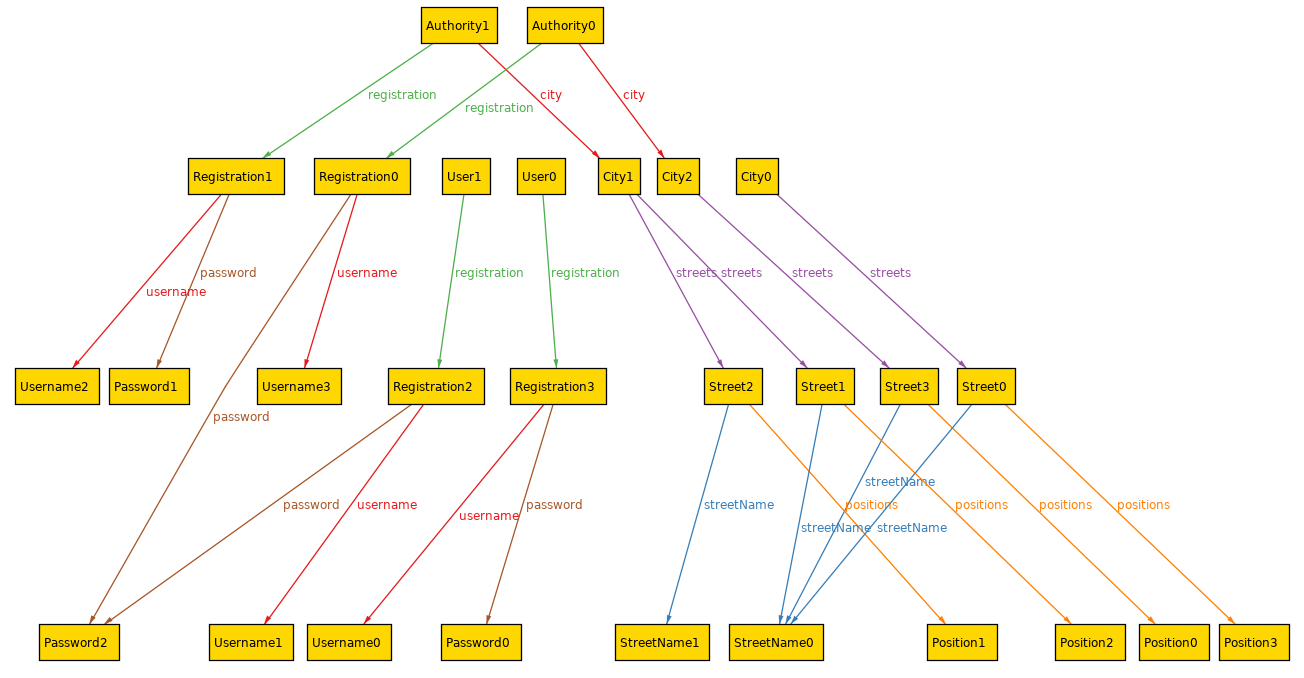
\includegraphics[scale=0.4, angle=90]{Files/alloy/world1.png}
		\caption{\label{fig:firstWorld}First World generated}
	\end{figure}
	
	\subsection[Second World]{\hyperlink{toc}{Second World}}
	%descrizione mondo
	This second world (\autoref{fig:secondWorld})captures a few aspects of the model: they are essentially reports, accidents and interventions. The threshold to activate the suggestion of an intervention has been lowered to 1 here. That means that if there's a report for a street, and that report has a violation type that is linked to an intervention, that intervention will be suggested by the system for that street. Alternatively, the same applies for accidents that are registered for a particular street. The two conditions for activating a suggested intervention are put in 'or'.
	The street name retrieved by the system while storing the report is of course the name of the street that contains the position that comes with that report.
	A stored report could be read by the authority. In case it's not, it will be part of the unread reports list for that authority.
	
	\begin{figure}[hbtp]
		\centering
		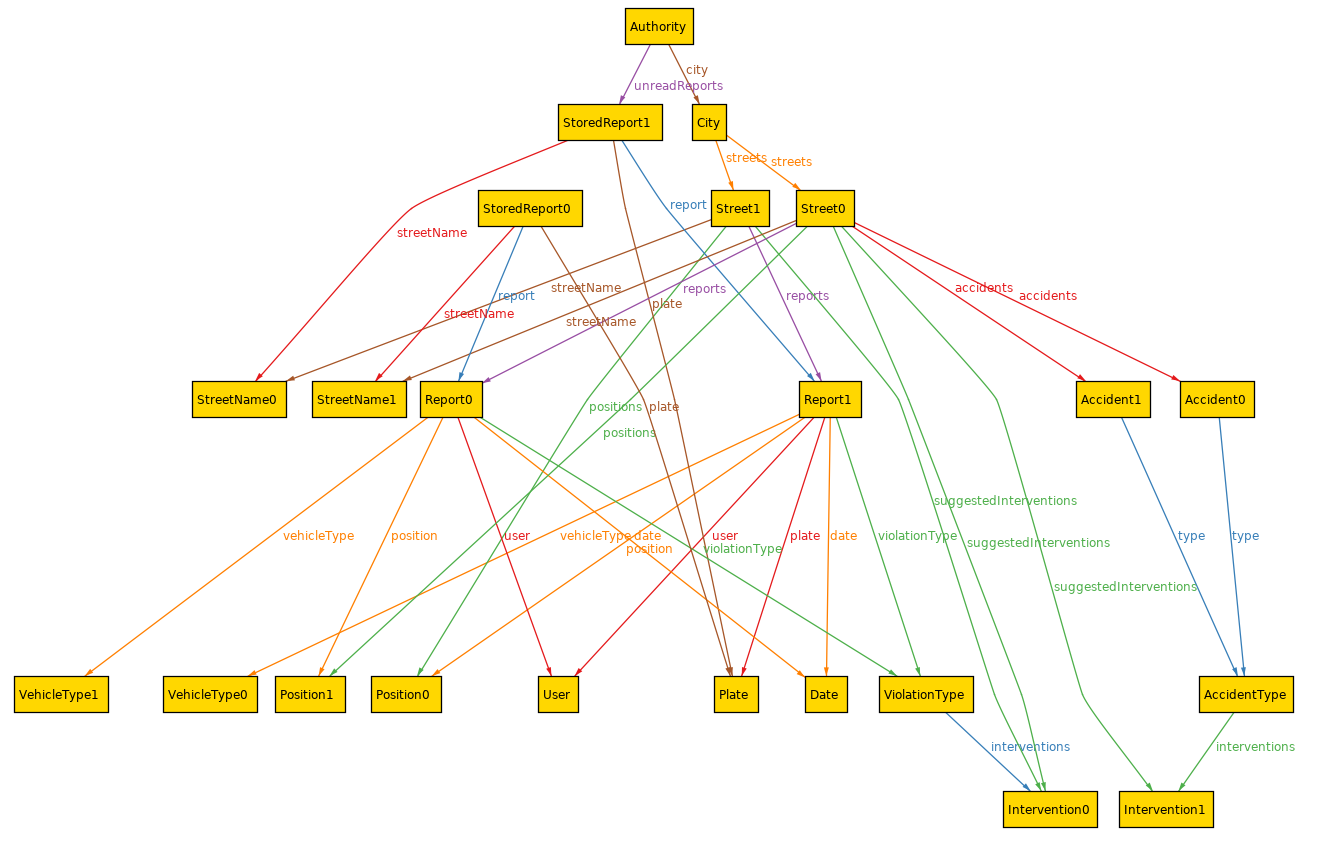
\includegraphics[scale=0.4, angle=90]{Files/alloy/world2.png}
		\caption{\label{fig:secondWorld}Second World Generated}
	\end{figure}
	
	\FloatBarrier
	\subsection[Third World]{\hyperlink{toc}{Third World}}
	%descrizione mondo
	This third and last example world focuses on the request mechanism. The use case is the one where a customer asks the system for possible interventions in a particular city. The result of that request will contain all the interventions suggested by the system, considering all the streets of the specified city.
	
	\begin{figure}[h!]
		\centering
		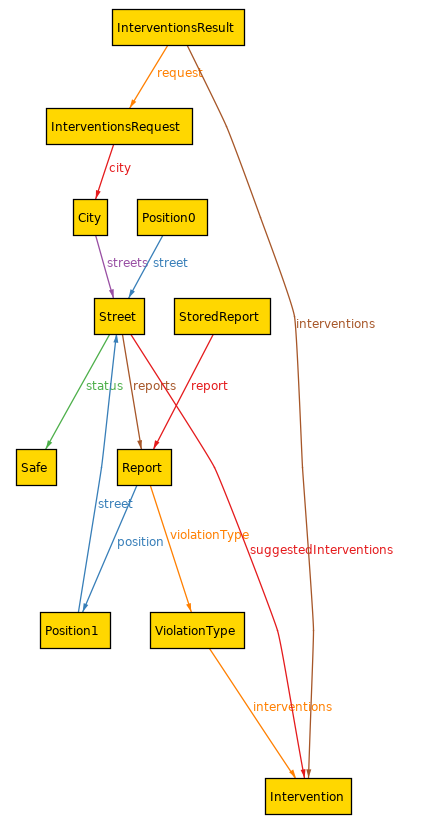
\includegraphics[scale=0.6]{Files/alloy/world3.png}
		\caption{Third World Generated}
	\end{figure}
	